
\section{\BookRecordIndex{T0125}分裂公理的证明}\label{sec:10-8}

先以略有不同但等价的形式重述\BookRecordIndex{T0125}分裂公理。以下始终假设 $(M,\omega)$ 是紧\BookRecordIndex{T0058}半正\BookRecordIndex{T0358}辛流形。
固定三个整数 $\ell^0,\ell^\infty\geq2$ 和 $k\geq\ell^0+\ell^\infty$，并记
\[
  I^0:=\{0,\ldots,\ell^0\},\qquad
  I^\infty:=\{0,\ldots,\ell^\infty\},\qquad
  I:=\{1,\ldots,\ell^0+\ell^\infty\}.
\]
这些集合为\BookRecordIndex{T0150}固定标记点 $\mathbf w$ 编号；前两个在先前的记号中对应
$I_{S_0},I_{S_1}$。令 $\mathcal S$ 表示指标集 $\{1,\ldots,k\}$ 的所有分裂
$S=(S^0,S^\infty)$ 所成的集合，其中
\[
  \{1,\ldots,\ell^0\}\subset S^0,
  \qquad
  \{\ell^0+1,\ldots,\ell^0+\ell^\infty\}\subset S^\infty.
\]
给定分裂 $S=(S^0,S^\infty)\in\mathcal S$，令
\[
  k^0:=k^0(S):=|S^0|\geq\ell^0,
  \qquad
  k^\infty:=k^\infty(S):=|S^\infty|\geq\ell^\infty,
\]
并以
\[
  \sigma^0:\{1,\ldots,k^0\}\longrightarrow\{1,\ldots,k\},
  \qquad
  \sigma^\infty:\{1,\ldots,k^\infty\}\longrightarrow\{1,\ldots,k\}
\]
表示满足 $\operatorname{im}\sigma^0=S^0$ 和
$\operatorname{im}\sigma^\infty=S^\infty$ 的唯一保序单射。因此，当
$1\leq i\leq\ell^0$ 时 $\sigma^0(i)=i$，而当
$1\leq i\leq\ell^\infty$ 时 $\sigma^\infty(i)=\ell^0+i$。用这些记号，
\BookRecordIndex{T0143}格罗莫夫--威滕不变量的\BookRecordIndex{T0125}分裂公理可表为如下形式。

\begin{theorem}[\BookRecordIndex{T0125}分裂公理]\label{thm:10-8-1}
对每个球面同调类 $A\in H_2(M;\mathbb Z)$ 和每一族上同调类
$a_1,\ldots,a_k\in H^*(M)$，有
\begin{align*}
  \operatorname{GW}_{A,k}^{M,I}(a_1,\ldots,a_k)
  ={}&\sum_{S\in\mathcal S}\sum_{A^0+A^\infty=A}
  \varepsilon(S,a)\varepsilon(S^0,a)\sum_{\nu,\mu}
  \operatorname{GW}_{A^0,k^0+1}^{M,I^0}
  \bigl(e_\nu,a_{\sigma^0(1)},\ldots,a_{\sigma^0(k^0)}\bigr)
  g^{\nu\mu}\\
  &\qquad{}\cdot
  \operatorname{GW}_{A^\infty,k^\infty+1}^{M,I^\infty}
  \bigl(e_\mu,a_{\sigma^\infty(1)},\ldots,
  a_{\sigma^\infty(k^\infty)}\bigr),
\end{align*}
其中 $e_\nu$ 构成 $H^*(M)$ 的一组基，
\[
  g_{\nu\mu}=\int_M e_\nu\smile e_\mu,
\]
$g^{\nu\mu}$ 是其逆矩阵，并且
\begin{align*}
  \varepsilon(S,a)
  &:={(-1)}^{\#\{(i,j)\in S^0\times S^\infty\mid
  j<i,\ \deg(a_i)\deg(a_j)\in2\mathbb Z+1\}},\\
  \varepsilon(S^0,a)
  &:={(-1)}^{\#\{i\in S^0\mid\deg(a_i)\in2\mathbb Z+1\}}.
\end{align*}
\end{theorem}

\begin{remark}\label{rem:10-8-2}
在定理~\ref{thm:10-8-1} 中，不变量
$\operatorname{GW}^{M,I^0}$ 和 $\operatorname{GW}^{M,I^\infty}$ 的\BookRecordIndex{T0066}标记点指标集分别
理解为 $\{0,\ldots,k^0\}$ 和 $\{0,\ldots,k^\infty\}$。
$\varepsilon(S,a)$ 的含义不变。额外符号 $\varepsilon(S^0,a)$ 的出现，是因为
类 $e_\nu$ 是 $\operatorname{GW}^{M,I^0}$ 的第一个而不是最后一个自变量。推导这个
符号公式时，我们使用了如下事实：$\operatorname{GW}^{M,I^0}$ 所取值的那些类的次数
之和总为偶数。
\end{remark}

\medskip
\noindent\textbf{\BookRecordIndex{T0226}连通对的\BookRecordIndex{T0283}求值映射。}
令 $\mathbf w^0=\{w_i^0\}_{1\leq i\leq\ell^0}$ 是
$S^2\setminus\{0\}$ 中两两不同的 $\ell^0$ 元组，令
$\mathbf w^\infty=\{w_j^\infty\}_{1\leq j\leq\ell^\infty}$ 是
$S^2\setminus\{\infty\}$ 中两两不同的 $\ell^\infty$ 元组。固定整数
$k\geq\ell^0+\ell^\infty$，取 $S=(S^0,S^\infty)\in\mathcal S$，记
\[
  k^0:=|S^0|,\qquad k^\infty:=|S^\infty|,
\]
并令 $\sigma^0,\sigma^\infty$ 如上为相应的重排映射。考虑\BookRecordIndex{T0246}模空间
\[
  \mathcal M_{0,S}(A^{0,\infty};\mathbf w^{0,\infty};J^{0,\infty})
  :=\mathcal M_{0,S}(A^0,A^\infty;
  \mathbf w^0,\mathbf w^\infty;J^0,J^\infty),
\]
它由所有元组
\[
  (u^0,u^\infty,\mathbf z^0,\mathbf z^\infty)
  =(u^0,u^\infty,z_1^0,\ldots,z_{k^0}^0,
  z_1^\infty,\ldots,z_{k^\infty}^\infty)
\]
组成，其中 $(u^0,u^\infty)\in\mathcal M(A^{0,\infty};J^{0,\infty})$，
$\mathbf z^0=\{z_i^0\}_{1\leq i\leq k^0}$ 是
$S^2\setminus\{0\}$ 中两两不同的 $k^0$ 元组，并满足下列条件
\sourcefootnote{原书把这里的指标上界印作 $\ell^\infty$；但
$\mathbf w^0$ 是 $\ell^0$ 元组，且本节前后固定在 $0$ 侧的恰为前
$\ell^0$ 个\BookRecordIndex{T0066}标记点，故补正为 $\ell^0$。}：
\[
  z_j^0=w_j^0,\qquad j=1,\ldots,\ell^0,
\]
而 $\mathbf z^\infty$ 的条件类似（见图~\ref{fig:10-8-3}）。与前面一样，假设
$J^0$ 和 $J^\infty$ 依赖于 $z$，从而无须限制到单纯映射。

\begin{figure}[tbp]
\centering
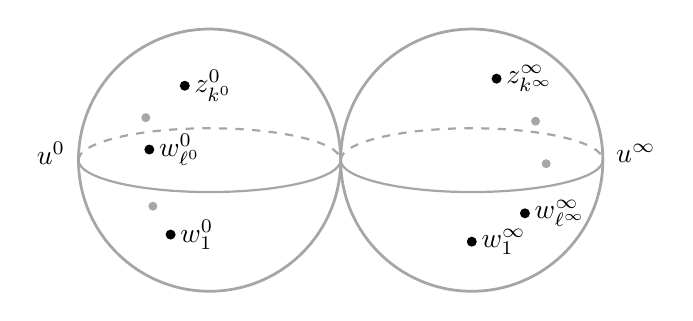
\begin{tikzpicture}[scale=.9]
  \draw[gray!70,line width=1pt] (-1.85,0) circle (1.85);
  \draw[gray!70,line width=1pt] (1.85,0) circle (1.85);
  \draw[gray!70,line width=.8pt] (-3.7,0) arc[start angle=180,end angle=360,x radius=1.85,y radius=.45];
  \draw[gray!70,dashed,line width=.8pt] (-3.7,0) arc[start angle=180,end angle=0,x radius=1.85,y radius=.45];
  \draw[gray!70,line width=.8pt] (0,0) arc[start angle=180,end angle=360,x radius=1.85,y radius=.45];
  \draw[gray!70,dashed,line width=.8pt] (0,0) arc[start angle=180,end angle=0,x radius=1.85,y radius=.45];
  \node[left] at (-3.75,.1) {$u^0$};
  \node[right] at (3.75,.1) {$u^\infty$};
  \fill (-2.2,1.05) circle (2pt) node[right] {$z_{k^0}^0$};
  \fill[gray!70] (-2.75,.6) circle (1.8pt);
  \fill (-2.7,.15) circle (2pt) node[right] {$w_{\ell^0}^0$};
  \fill (-2.4,-1.05) circle (2pt) node[right] {$w_1^0$};
  \fill[gray!70] (-2.65,-.65) circle (1.8pt);
  \fill (2.2,1.15) circle (2pt) node[right] {$z_{k^\infty}^\infty$};
  \fill[gray!70] (2.75,.55) circle (1.8pt);
  \fill[gray!70] (2.9,-.05) circle (1.8pt);
  \fill (2.6,-.75) circle (2pt) node[right] {$w_{\ell^\infty}^\infty$};
  \fill (1.85,-1.15) circle (2pt) node[right] {$w_1^\infty$};
\end{tikzpicture}
\caption{带\BookRecordIndex{T0066}标记点的\BookRecordIndex{T0226}连通对。}\label{fig:10-8-3}
\end{figure}

这个空间带有\BookRecordIndex{T0283}求值映射
\[
  \operatorname{ev}_{A^{0,\infty},S}:
  \mathcal M_{0,S}(A^{0,\infty};\mathbf w^{0,\infty};J^{0,\infty})
  \longrightarrow M^k,
\]
其定义为
$\operatorname{ev}_S(u^0,u^\infty,\mathbf z^0,\mathbf z^\infty)
:=(x_1,\ldots,x_k)$，其中
\[
  x_{\sigma^0(i)}:=u^0(z_i^0),\qquad
  x_{\sigma^\infty(j)}:=u^\infty(z_j^\infty),
\]
$i=1,\ldots,k^0$，$j=1,\ldots,k^\infty$。还要考虑这个\BookRecordIndex{T0283}求值映射在紧子集
\[
  \mathcal M_{0,S}(A^{0,\infty};\mathbf w^{0,\infty};J^{0,\infty},c)
  \subset
  \mathcal M_{0,S}(A^{0,\infty};\mathbf w^{0,\infty};J^{0,\infty})
\]
上的限制；该紧子集由所有满足
\[
  \lVert du^0\rVert_{L^\infty}\leq c,\qquad
  \lVert du^\infty\rVert_{L^\infty}\leq c
\]
以及
\[
  |z_i^0-z_{i'}^0|\geq\frac1c,\qquad
  |z_i^0|\geq\frac1c,\qquad
  |z_j^\infty-z_{j'}^\infty|\geq\frac1c,\qquad
  |z_j^\infty|\leq c
\]
的元组组成，其中 $i\ne i'$、$j\ne j'$。下一个推论立即来自
定理~\ref{thm:10-1-2} 第（iii）部分。

\begin{corollary}\label{cor:10-8-3}
固定两个同调类 $A^0,A^\infty\in H_2(M;\mathbb Z)$、一个\BookRecordIndex{T0088}殆复结构\BookRecordIndex{T0406}正则对
\[
  (J^0,J^\infty)\in\mathcal J_{\mathrm{reg}}(S^2;A^{0,\infty})
\]
以及常数 $c>0$。令 $A:=A^0+A^\infty$，并令
$\delta_0=\delta_0(c)$ 为定理~\ref{thm:10-1-2} 中的常数。假设
$0<\delta<\delta_0$，且对 $R>1/(\delta\delta_0)$，令
\[
  \iota_c^R=\iota_c^{\delta,R}:
  \mathcal M(A^{0,\infty};J^{0,\infty},c)
  \longrightarrow\mathcal M(A;J^R)
\]
为定理~\ref{thm:10-1-2} 中引入的映射。令
$\mathbf w^0=\{w_i^0\}_{1\leq i\leq\ell^0}$ 是
$S^2\setminus\{0\}$ 中两两不同的 $\ell^0$ 元组，令
$\mathbf w^\infty=\{w_j^\infty\}_{1\leq j\leq\ell^\infty}$ 是
$S^2\setminus\{\infty\}$ 中两两不同的 $\ell^\infty$ 元组。固定整数
$k\geq\ell^0+\ell^\infty$，取 $S=(S^0,S^\infty)\in\mathcal S$，并定义
\[
  w_i^R:=w_i^0\quad(i=1,\ldots,\ell^0),
  \qquad
  w_{\ell^0+j}^R:=w_j^\infty/R^2
  \quad(j=1,\ldots,\ell^\infty).
\]
考虑嵌入
\[
  \iota_{c,S}^R:
  \mathcal M_{0,S}(A^{0,\infty};\mathbf w^{0,\infty};J^{0,\infty},c)
  \longrightarrow
  \mathcal M_{0,k}^*(A;\mathbf w^R;J^R),
\]
它由
\[
  \iota_{c,S}^R(u^0,u^\infty,\mathbf z^0,\mathbf z^\infty)
  :=(\widetilde u^R,\mathbf z^R)
\]
给出，其中
\[
  \widetilde u^R:=\iota_c^R(u^0,u^\infty),
  \qquad z_{\sigma^0(i)}^R:=z_i^0,
  \qquad z_{\sigma^\infty(j)}^R:=z_j^\infty/R^2
\]
（$i=1,\ldots,k^0$，$j=1,\ldots,k^\infty$）。则当 $R$ 趋于无穷时，
\BookRecordIndex{T0283}求值映射
\[
  \operatorname{ev}^R:\mathcal M_{0,k}^*(A;\mathbf w^R;J^R)\longrightarrow M^k
\]
与 $\iota_{c,S}^R$ 的复合在 $C^1$ 拓扑下收敛到
$\operatorname{ev}_{A^{0,\infty},S}$。
\end{corollary}

\medskip
\noindent\textbf{\BookRecordIndex{T0226}连通对\BookRecordIndex{T0246}模空间的极限集。}
证明定理~\ref{thm:10-8-1} 的第一步，是说明\BookRecordIndex{T0283}求值映射
\[
  \operatorname{ev}_{A^{0,\infty},S}:
  \mathcal M_{0,S}^*(A^{0,\infty};\mathbf w^{0,\infty};J^{0,\infty})
  \longrightarrow M^k
\]
是一个\BookRecordIndex{T0337}伪循环。其证明与说明\BookRecordIndex{T0084}带标号树 $T$ 上的\BookRecordIndex{T0340}稳定映射的\BookRecordIndex{T0283}求值映射
\[
  \operatorname{ev}_T:\mathcal M_{0,T}^*(\{A_\alpha\};J)\longrightarrow M^k
\]
为\BookRecordIndex{T0337}伪循环时所需的证明几乎相同；见习题~\ref{ex:6-6-3}。不过，$J^0$ 和
$J^\infty$ 对 $z$ 的依赖带来了一些额外特征，下面对此加以说明。

第一步是理解定义域中\BookRecordIndex{T0141}格罗莫夫收敛序列的极限。由于 $J^0$ 和 $J^\infty$ 随定义域
$S^2$ 上的点变化，这些极限是带两个特殊分支的\BookRecordIndex{T0340}稳定映射：这两个分支分别标为 $0$ 和
$\infty$，并分别关于 $\{J_z^0\}$ 和 $\{J_z^\infty\}$ 全纯。其余分支都是\BookRecordIndex{T0275}气泡；
它们关于固定复结构 $J_{z_\alpha}^0$ 或 $J_{z_\alpha}^\infty$ 全纯，该复结构对应于
它们附着到某个特殊分支的点。与第~\ref{sec:6-7} 节一样，把问题看成
$u^0,u^\infty$ 的图像 $\widetilde u^0,\widetilde u^\infty$ 的收敛很有用。
但现在两个主分支之间也可能形成\BookRecordIndex{T0275}气泡。因此，极限还有第三部分，它关于式~\eqref{eq:10-1-1}
中与 $u^0$ 到 $u^\infty$ 的附着点相联系的 $J$ 全纯。稍后我们会更精确地表述上述讨论；
目前它只是为了引出下面的定义。

令 $\mathbf w^0=\{w_i^0\}_{1\leq i\leq\ell^0}$ 和
$\mathbf w^\infty=\{w_j^\infty\}_{1\leq j\leq\ell^\infty}$ 是 $S^2$ 上两两
不同的点的元组，并且对所有 $i,j$ 都有 $w_i^0\ne0$、$w_j^\infty\ne\infty$。
令 $T=(T,E,\Lambda)$ 是一棵带 $k$ 个标号的树，具有两个不同的\BookRecordIndex{T0321}特殊顶点
$0$ 和 $\infty$。定义\BookRecordIndex{T0417}子树 $T^0,T^\infty\subset T$ 为
\[
  T^0:=\{\alpha\in T\mid0\in[\alpha,\infty]\},
  \qquad
  T^\infty:=\{\alpha\in T\mid\infty\in[0,\alpha]\}.
\]
换言之，从 $0$ 沿指向 $\infty$ 的方向切去分支便得到 $T^0$，从 $\infty$ 沿指向
$0$ 的方向切去分支便得到 $T^\infty$。假设标号满足
\[
  \alpha_i\in T^0\quad(i=1,\ldots,\ell^0),
  \qquad
  \alpha_{\ell^0+j}\in T^\infty\quad(j=1,\ldots,\ell^\infty)
\]
（见图~\ref{fig:10-8-4}）。

固定一族同调类 $\mathbf B=\{B_\alpha\}_{\alpha\in T}\subset H_2(M;\mathbb Z)$，
并假设 $J^0,J^\infty$ 满足式~\eqref{eq:10-1-1}。\BookRecordIndex{T0246}模空间
\[
  \mathcal M_{0,T}^*(\{B_\alpha\};\mathbf w^{0,\infty};J^{0,\infty})
\]
由元组
\[
\begin{split}
  (\mathbf u,\mathbf z):={}&
  \bigl(u_0,u_\infty,
  \{z_\alpha,u_\alpha\}_{\alpha\in(T^0\cup T^\infty)\setminus\{0,\infty\}},\\
  &\{u_\alpha\}_{\alpha\in T\setminus(T^0\cup T^\infty)},
  \{z_{\alpha\beta}\}_{\alpha E\beta},
  \{\alpha_i,z_i\}_{1\leq i\leq k}\bigr)
\end{split}
\]
组成，并满足以下条件。

\begin{description}
\item[（映射）]
每个 $u_\alpha:S^2\to M$ 都是表示类 $B_\alpha$ 的光滑映射。此外，$u_0$ 是
$\{J_z^0\}$-全纯球面，$u_\infty$ 是 $\{J_z^\infty\}$-全纯球面；当
$\alpha\in T^0\setminus\{0\}$ 时，$u_\alpha$ 是 $J_{z_\alpha}^0$-全纯球面；
当 $\alpha\in T^\infty\setminus\{\infty\}$ 时，$u_\alpha$ 是
$J_{z_\alpha}^\infty$-全纯球面；当
$\alpha\in T\setminus(T^0\cup T^\infty)$ 时，$u_\alpha$ 是 $J$-全纯球面。

\item[（\BookRecordIndex{T0191}节点）]
若 $\alpha E\beta$，则
$u_\alpha(z_{\alpha\beta})=u_\beta(z_{\beta\alpha})$。此外，当
$\alpha E\beta$ 且 $\alpha,\beta\in T^0\setminus\{0\}$，或
$\alpha,\beta\in T^\infty\setminus\{\infty\}$ 时，有 $z_\alpha=z_\beta$。
若 $0E\alpha$ 且 $\infty E\beta$，则
\[
  z_{0\alpha}=\begin{cases}
    z_\alpha,&\alpha\in T^0,\\
    0,&\alpha\notin T^0,
  \end{cases}
  \qquad
  z_{\infty\beta}=\begin{cases}
    z_\beta,&\beta\in T^\infty,\\
    \infty,&\beta\notin T^\infty.
  \end{cases}
\]

\item[（稳定性）]
对 $\alpha E\beta$ 的点 $z_{\alpha\beta}$ 与对 $\alpha_i=\alpha$ 的点 $z_i$
两两不同；只要 $u_\alpha$ 为常值且 $\alpha\ne0,\infty$，这样的点至少有三个。

\item[（固定）]
若 $i\in\{1,\ldots,\ell^0\}$、$j\in\{1,\ldots,\ell^\infty\}$，则
\sourcefootnote{原书在右侧两个分支条件中把顶点下标印作 $\alpha_j$；但此处所固定的是
第 $\ell^0+j$ 个\BookRecordIndex{T0066}标记点，且同一分式的分子已经分别写成
$z_{\ell^0+j}$ 和 $z_{\alpha_{\ell^0+j}}$，故补正为 $\alpha_{\ell^0+j}$。}
\[
  w_i^0=\begin{cases}
    z_i,&\alpha_i=0,\\
    z_{\alpha_i},&\alpha_i\ne0,
  \end{cases}
  \qquad
  w_j^\infty=\begin{cases}
    z_{\ell^0+j},&\alpha_{\ell^0+j}=\infty,\\
    z_{\alpha_{\ell^0+j}},&\alpha_{\ell^0+j}\ne\infty.
  \end{cases}
\]

\item[（单纯）]
对每个 $z\in S^2$，\BookRecordIndex{T0417}子树
\[
  T_z^0:=\{\alpha\in T^0\mid z_\alpha=z\},
  \qquad
  T_z^\infty:=\{\alpha\in T^\infty\mid z_\alpha=z\}
\]
上的\BookRecordIndex{T0340}稳定映射都是单纯的，而\BookRecordIndex{T0417}子树 $T\setminus(T^0\cup T^\infty)$ 上的\BookRecordIndex{T0340}稳定映射也是
单纯的。
\end{description}

\begin{figure}[tbp]
\centering
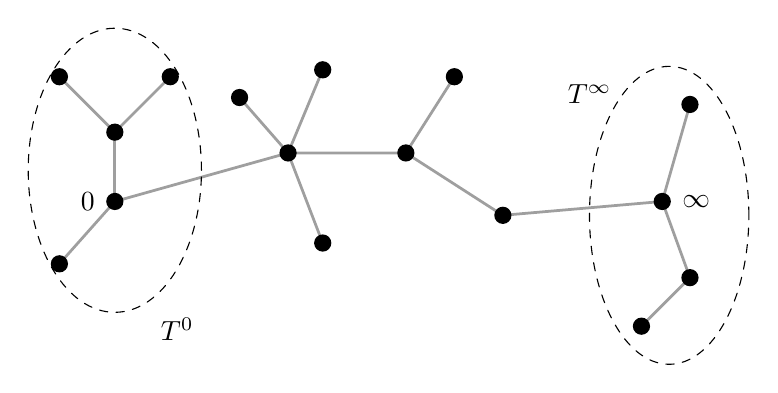
\begin{tikzpicture}[scale=.88,line cap=round,line join=round]
  \tikzset{v/.style={circle,fill,inner sep=2.2pt}}
  \draw[gray!75,line width=1pt]
    (-4,0)--(-1.5,.7)--(.2,.7)--(1.6,-.2)--(3.9,0);
  \draw[gray!75,line width=1pt] (-4,0)--(-4.8,-.9);
  \draw[gray!75,line width=1pt] (-4,0)--(-4,1);
  \draw[gray!75,line width=1pt] (-4,1)--(-4.8,1.8);
  \draw[gray!75,line width=1pt] (-4,1)--(-3.2,1.8);
  \draw[gray!75,line width=1pt] (-1.5,.7)--(-2.2,1.5);
  \draw[gray!75,line width=1pt] (-1.5,.7)--(-1,1.9);
  \draw[gray!75,line width=1pt] (-1.5,.7)--(-1,-.6);
  \draw[gray!75,line width=1pt] (.2,.7)--(.9,1.8);
  \draw[gray!75,line width=1pt] (3.9,0)--(4.3,1.4);
  \draw[gray!75,line width=1pt] (3.9,0)--(4.3,-1.1)--(3.6,-1.8);
  \foreach \p in {(-4,0),(-4.8,-.9),(-4,1),(-4.8,1.8),(-3.2,1.8),
    (-1.5,.7),(-2.2,1.5),(-1,1.9),(-1,-.6),(.2,.7),(.9,1.8),(1.6,-.2),
    (3.9,0),(4.3,1.4),(4.3,-1.1),(3.6,-1.8)}
    \node[v] at \p {};
  \draw[dashed] (-4,.45) ellipse (1.25 and 2.05);
  \draw[dashed] (4,-.2) ellipse (1.15 and 2.15);
  \node[left] at (-4.15,0) {$0$};
  \node[right] at (4.05,0) {$\infty$};
  \node at (-3.1,-1.85) {$T^0$};
  \node at (2.85,1.55) {$T^\infty$};
\end{tikzpicture}
\caption{带两个\BookRecordIndex{T0321}特殊顶点的\BookRecordIndex{T0275}气泡树。}\label{fig:10-8-4}
\end{figure}

为理解这一定义，考虑图像
$\widetilde u_0(z):=(z,u_0(z))$，把它看作
$\widetilde M:=S^2\times M$ 的一个 $\widetilde J^0$-全纯截面。这里
$\widetilde J^0$ 表示如下\BookRecordIndex{T0088}殆复结构：它在每个水平子空间
$T_zS^2\times\{0\}$ 上等于标准复结构，并且在嵌入
\[
  \iota_z:M\longrightarrow\widetilde M,
  \qquad \iota_z(x):=(z,x)
\]
下拉回为 $J_z^0$。对 $\alpha\in T^0\setminus\{0\}$，偶对
$(z_\alpha,u_\alpha)$ 给出竖直 $\widetilde J^0$-全纯球面
$\widetilde u_\alpha(z):=(z_\alpha,u_\alpha(z))$。用这些记号，（映射）、（\BookRecordIndex{T0191}节点）和
（稳定性）条件断言 $(\mathbf u,\mathbf z)$ 在\BookRecordIndex{T0417}子树 $T^0$ 上的限制是
$(\widetilde M,\widetilde J^0)$ 中的\BookRecordIndex{T0340}稳定映射。同样，它在 $T^\infty$ 上的限制是
$(\widetilde M,\widetilde J^\infty)$ 中的\BookRecordIndex{T0340}稳定映射。这两个\BookRecordIndex{T0340}稳定映射通过
$(M,J)$ 中的第三个\BookRecordIndex{T0340}稳定映射相连；后者以\BookRecordIndex{T0417}子树 $T\setminus(T^0\cup T^\infty)$ 为模型。
（固定）条件断言前 $\ell^0$ 个\BookRecordIndex{T0066}标记点属于 $T^0$ 并投影到点 $w_i^0$，接下来的
$\ell^\infty$ 个\BookRecordIndex{T0066}标记点属于 $T^\infty$ 并投影到点 $w_j^\infty$。

最后一个条件断言该\BookRecordIndex{T0340}稳定映射是单纯的。与第 6 章一样，这是对一般\BookRecordIndex{T0088}殆复结构族获得\BookRecordIndex{T0166}横截性所
必需的。事实上，与定理~\ref{thm:6-7-11} 的证明相同，可以选取\BookRecordIndex{T0088}殆复结构
$J$、$\{J_z^0\}_{z\in S^2}$ 和 $\{J_z^\infty\}_{z\in S^2}$，使
式~\eqref{eq:10-1-1} 成立，且所有相关的\BookRecordIndex{T0065}边求值映射都横截于相应的\BookRecordIndex{T0061}边对角线。因此每个
\BookRecordIndex{T0246}模空间
\[
  \mathcal M_{0,T}^*(\{B_\alpha\};\mathbf w^{0,\infty};J^{0,\infty})
\]
都是维数为
\[
  \dim\mathcal M_{0,T}^*(\{B_\alpha\};\mathbf w^{0,\infty};J^{0,\infty})
  =2n+2c_1(B)+2(k-\ell^0-\ell^\infty)-2(e(T)-1)
\]
的光滑流形，其中 $B:=\sum_{\alpha\in T}B_\alpha$。该\BookRecordIndex{T0246}模空间带有\BookRecordIndex{T0283}求值映射
\[
  \operatorname{ev}_{\{B_\alpha\},T}:
  \mathcal M_{0,T}^*(\{B_\alpha\};\mathbf w^{0,\infty};J^{0,\infty})
  \longrightarrow M^k,
\]
其定义为
\[
  \operatorname{ev}_{\{B_\alpha\},T}(\mathbf u,\mathbf z)
  :=\bigl(u_{\alpha_1}(z_1),\ldots,u_{\alpha_k}(z_k)\bigr).
\]
注意，$\operatorname{ev}_{A^{0,\infty},S}$ 对应于如下特殊情形：树 $T$ 恰有两个顶点
$0,\infty$，且标号由 $i\in S^0$ 时 $\alpha_i=0$、$i\in S^\infty$ 时
$\alpha_i=\infty$ 给出。对上述 $J,J^0,J^\infty$ 的选择，与
定理~\ref{thm:6-7-1} 的证明相同，\BookRecordIndex{T0283}求值映射
\[
  \operatorname{ev}_{A^{0,\infty},S}:
  \mathcal M_{0,S}(A^{0,\infty};\mathbf w^{0,\infty};J^{0,\infty})
  \longrightarrow M^k
\]
对所有类 $A^0,A^\infty$ 和所有分裂 $S\in\mathcal S$ 都是\BookRecordIndex{T0337}伪循环。

\begin{proof}[定理~\ref{thm:10-8-1} 的证明]
不妨假设上同调类 $a_i$ 是紧定向光滑子流形 $X_i\subset M$ 的庞加莱对偶：
\[
  a_i=\operatorname{PD}([X_i]).
\]
对 $a_i$ 取适当的整数倍后，这总能做到。引理~\ref{lem:6-5-5} 证明中的\BookRecordIndex{T0166}横截性论证说明，
可以选取子流形 $X_i$，使其乘积
\[
  \mathbf X:=X_1\times\cdots\times X_k\subset M^k
\]
横截于上面讨论的每个\BookRecordIndex{T0283}求值映射 $\operatorname{ev}_{\{B_\alpha\},T}$。于是，对每个
分裂 $S\in\mathcal S$ 和每对同调类
$A^0,A^\infty\in H_2(M;\mathbb Z)$，\BookRecordIndex{T0337}伪循环 $\mathbf X$ 都与\BookRecordIndex{T0283}求值映射
$\operatorname{ev}_{A^{0,\infty},S}$ \BookRecordIndex{T0281}强横截。

我们断言
\begin{align}
  \mathbf X\mathbin{\cdot}\operatorname{ev}_{A^{0,\infty},S}
  ={}&\varepsilon(S,a)\varepsilon(S^0,a)\sum_{\nu,\mu}
  \operatorname{GW}_{A^0,k^0+1}^{M,I^0}
  \bigl(e_\nu,a_{\sigma^0(1)},\ldots,a_{\sigma^0(k^0)}\bigr)
  g^{\nu\mu}\notag\\
  &\qquad{}\cdot
  \operatorname{GW}_{A^\infty,k^\infty+1}^{M,I^\infty}
  \bigl(e_\mu,a_{\sigma^\infty(1)},\ldots,
  a_{\sigma^\infty(k^\infty)}\bigr).
  \label{eq:10-8-1}
\end{align}
为说明这一点，考虑由所有元组
\[
  (\mathbf u,\mathbf z):=(u^0,u^\infty,\mathbf z^0,\mathbf z^\infty)
\]
组成的\BookRecordIndex{T0246}模空间 $\widehat{\mathcal M}(A^{0,\infty},S)$；它们满足\BookRecordIndex{T0246}模空间
$\mathcal M_{0,S}(A^{0,\infty};\mathbf w^{0,\infty};J^{0,\infty})$ 的全部条件，
唯一的例外是不要求 $u^0(0)=u^\infty(\infty)$。该空间带有\BookRecordIndex{T0283}求值映射
\[
  \widehat{\operatorname{ev}}_{A^{0,\infty},S}:
  \widehat{\mathcal M}(A^{0,\infty},S)
  \longrightarrow M^k\times M\times M,
\]
其定义为
\[
  \widehat{\operatorname{ev}}_{A^{0,\infty},S}(\mathbf u,\mathbf z)
  :=\bigl(\operatorname{ev}_{A^{0,\infty},S}(\mathbf u,\mathbf z),
  u^0(0),u^\infty(\infty)\bigr).
\]
我们的假设保证 $\widehat{\operatorname{ev}}_{A^{0,\infty},S}$ 是\BookRecordIndex{T0337}伪循环，而且
式~\eqref{eq:10-8-1} 左端等于该\BookRecordIndex{T0337}伪循环与乘积 $\mathbf X\times\Delta$ 的交数，其中
$\Delta\subset M\times M$ 是对角线：
\[
  \mathbf X\mathbin{\cdot}\operatorname{ev}_{A^{0,\infty},S}
  =(\mathbf X\times\Delta)\mathbin{\cdot}
  \widehat{\operatorname{ev}}_{A^{0,\infty},S}.
\]
对角线同调类的庞加莱对偶为
\begin{equation}\label{eq:10-8-2}
  \operatorname{PD}([\Delta])
  =\sum_{\nu,\mu}g^{\nu\mu}\pi_1^*e_\nu\smile\pi_2^*e_\mu,
\end{equation}
其中 $\pi_1,\pi_2:M\times M\to M$ 是自然投影。考察靶空间中相应置换所带来的符号
变化，便由此得到式~\eqref{eq:10-8-1}。

由式~\eqref{eq:10-8-1}，定理~\ref{thm:10-8-1} 的断言可写为
\begin{equation}\label{eq:10-8-3}
  \operatorname{GW}_{A,k}^{M,I}(a_1,\ldots,a_k)
  =\sum_{S\in\mathcal S}\sum_{A^0+A^\infty=A}
  \mathbf X\mathbin{\cdot}\operatorname{ev}_{A^{0,\infty},S}.
\end{equation}
现在用推论~\ref{cor:10-1-4} 和推论~\ref{cor:10-8-3} 证明这个等式。

记
\[
  \mathcal M^{0,\infty}(\mathbf X):=
  \bigcup_{\substack{A^0+A^\infty=A\\S\in\mathcal S}}
  \operatorname{ev}_{A^{0,\infty},S}^{-1}(\mathbf X),
\]
即所有元组
\[
  (\mathbf u,\mathbf z):=(u^0,u^\infty,\mathbf z^0,\mathbf z^\infty)
  \in\mathcal M_{0,S}(A^{0,\infty};\mathbf w^{0,\infty};J^{0,\infty})
\]
所成的集合；这里 $S$ 遍历 $\mathcal S$ 中所有分裂，$A^0,A^\infty$ 遍历所有满足
$A^0+A^\infty=A$ 的同调类，并且
$\operatorname{ev}_{A^{0,\infty},S}(\mathbf u,\mathbf z)\in\mathbf X$。类似地，记
\[
  \mathcal M^R(\mathbf X):=(\operatorname{ev}^R)^{-1}(\mathbf X)
  \subset\mathcal M_{0,k}(A;\mathbf w^R;J^R)
\]
为所有满足
$\operatorname{ev}^R(v^R,\mathbf z^R)\in\mathbf X$ 的元组
$(v^R,\mathbf z^R)\in\mathcal M_{0,k}(A;\mathbf w^R;J^R)$ 所成的集合。

依假设，$\mathcal M^{0,\infty}(\mathbf X)$ 是有限集，所以可以把常数 $c$ 取得充分大，
使该集合的每个元素都属于某个紧子集
\[
  \mathcal M_{0,S}(A^{0,\infty};\mathbf w^{0,\infty};J^{0,\infty},c-1).
\]
$\mathbf X$ 的\BookRecordIndex{T0166}横截性假设与推论~\ref{cor:10-8-3} 中\BookRecordIndex{T0283}求值映射的 $C^1$ 收敛说明，
每个这样的解都给出唯一的邻近元素
$(v^R,\mathbf z^R)\in\mathcal M_{0,k}(A;\mathbf w^R;J^R)$；它满足
$\operatorname{ev}^R(v^R,\mathbf z^R)\in\mathbf X$，并对不变量贡献相同的符号。
注意，映射 $v^R$ 一般不等于\BookRecordIndex{T0254}粘合
$\widetilde u^R:=\iota_c^R(\mathbf u)$，因为 $\widetilde u^R$ 的像未必在具有正确\BookRecordIndex{T0185}交比的
点处与 $\mathbf X$ 相交。不过，$v^R$ 会非常接近这个\BookRecordIndex{T0254}粘合。更准确地说，当 $R$ 充分大时，
存在唯一单射
\begin{equation}\label{eq:10-8-4}
  \mathcal T^R:\mathcal M^{0,\infty}(\mathbf X)
  \longrightarrow\mathcal M^R(\mathbf X),
\end{equation}
其定义如下。若
\[
  (\mathbf u,\mathbf z)\in\mathcal M^{0,\infty}(\mathbf X)
  \cap\mathcal M_{0,S}(A^{0,\infty};\mathbf w^{0,\infty};J^{0,\infty},c-1),
\]
则存在唯一的邻近元素
\[
  (\mathbf u',\mathbf z')
  \in\mathcal M_{0,S}(A^{0,\infty};\mathbf w^{0,\infty};J^{0,\infty},c)
\]
满足 $\operatorname{ev}^R\circ\iota_{c,S}^R(\mathbf u',\mathbf z')
\in\mathbf X$；于是定义
\[
  \mathcal T^R(\mathbf u,\mathbf z):=
  \iota_{c,S}^R(\mathbf u',\mathbf z')\in\mathcal M^R(\mathbf X).
\]

还须证明，当 $R$ 充分大时 $\mathcal T^R$ 满射。反设不然，则存在序列
$R_\nu\to\infty$，使 $\mathcal T^{R_\nu}$ 不是满射。取不属于
$\mathcal T^{R_\nu}$ 的像的元素
$(u_\nu,\mathbf z_\nu)\in\mathcal M^{R_\nu}(\mathbf X)$。我们断言
\begin{equation}\label{eq:10-8-5}
  \forall c>0,\quad\exists\nu_c\in\mathbb N,\quad
  \forall\nu\geq\nu_c,\quad
  (u_\nu,\mathbf z_\nu)\notin\operatorname{im}\iota_{c,S}^{R_\nu}.
\end{equation}
否则，存在常数 $c>0$、序列 $\nu_i\to\infty$、分裂 $S\in\mathcal S$、一对满足
$A^0+A^\infty=A$ 的同调类 $A^0,A^\infty\in H_2(M;\mathbb Z)$，以及序列
\[
  (\mathbf u_i,\mathbf z_i):=
  (u_i^0,u_i^\infty,\mathbf z_i^0,\mathbf z_i^\infty)
  \in\mathcal M_{0,S}(A^{0,\infty};\mathbf w^{0,\infty};J^{0,\infty},c),
\]
使得对每个 $i$ 都有
\[
  (u_{\nu_i},\mathbf z_{\nu_i})
  =\iota_{c,S}^{R_{\nu_i}}(\mathbf u_i,\mathbf z_i).
\]
由于 $(u_{\nu_i},\mathbf z_{\nu_i})\in\mathcal M^{R_{\nu_i}}(\mathbf X)$，
对每个 $i$ 都有
\[
  \operatorname{ev}^{R_{\nu_i}}\circ
  \iota_{c,S}^{R_{\nu_i}}(\mathbf u_i,\mathbf z_i)\in\mathbf X.
\]
又由于
$\mathcal M_{0,S}(A^{0,\infty};\mathbf w^{0,\infty};J^{0,\infty},c)$ 紧，必要时取子列，
可以假设 $(\mathbf u_i,\mathbf z_i)$ 收敛到
\[
  (\mathbf u,\mathbf z)
  \in\mathcal M_{0,S}(A^{0,\infty};\mathbf w^{0,\infty};J^{0,\infty},c).
\]
由推论~\ref{cor:10-8-3}，这个极限必属于
$\mathcal M^{0,\infty}(\mathbf X)$。于是根据式~\eqref{eq:10-8-4} 中
$\mathcal T^{R_{\nu_i}}$ 的定义，当 $i$ 充分大时
\[
  (u_{\nu_i},\mathbf z_{\nu_i})
  =\mathcal T^{R_{\nu_i}}(\mathbf u,\mathbf z),
\]
这与我们对原序列 $(u_{\nu_i},\mathbf z_{\nu_i})$ 的假设矛盾。因此
式~\eqref{eq:10-8-5} 得证。

现在由式~\eqref{eq:10-8-5} 和推论~\ref{cor:10-1-4}，
$(u_\nu,\mathbf z_\nu)$ 有一个子列\BookRecordIndex{T0141}格罗莫夫收敛到穿过 $\mathbf X$、具有多于两个分支的
\BookRecordIndex{T0340}稳定映射。更准确地说，取子列后，可以假设 $u_\nu(z)$ \BookRecordIndex{T0247}模冒泡收敛到
$S^2\setminus\{0\}$ 上的 $\{J_z^0\}$-全纯球面 $u^0$，而
$u_\nu(z/R_\nu^2)$ \BookRecordIndex{T0247}模冒泡收敛到 $S^2\setminus\{\infty\}$ 上的
$\{J_z^\infty\}$-全纯球面 $u^\infty$。第二个极限存在这一事实来自 $J^R$ 的定义。

为理解极限\BookRecordIndex{T0340}稳定映射，必须区分定理~\ref{thm:5-3-1} 证明中的三种情形。具体而言，
极限中除 $u^0$ 外的每个分支都是形如
$u_\nu(z_\nu+\varepsilon_\nu z)$ 的序列的极限，其中 $z_\nu$ 收敛到 $S^2$ 中一点，
$\varepsilon_\nu$ 收敛到零；参见命题~\ref{prop:4-7-1} 的证明，它是
定理~\ref{thm:5-3-1} 证明的主要步骤。这三种情形是
\begin{description}
\item[情形 1：] $\displaystyle\lim_{\nu\to\infty}|z_\nu|>0$；
\item[情形 2：] $\displaystyle\lim_{\nu\to\infty}|z_\nu|=0$ 且
$\displaystyle\lim_{\nu\to\infty}R_\nu^2|z_\nu|=\infty$；
\item[情形 3：] $\displaystyle\lim_{\nu\to\infty}R_\nu^2|z_\nu|<\infty$。
\end{description}
在第一种情形，极限\BookRecordIndex{T0340}稳定映射的相应分支属于\BookRecordIndex{T0417}子树 $T^0$；在第三种情形，它属于
$T^\infty$；在居中的第二种情形，它属于补集 $T\setminus(T^0\cup T^\infty)$。

我们断言，极限\BookRecordIndex{T0340}稳定映射以一棵具有多于两个顶点的树为模型。它至少有两个顶点，即标为
$0$ 和 $\infty$ 的顶点。事实上，若
\[
  [u^0]+[u^\infty]\ne A,
\]
则极限有非常值\BookRecordIndex{T0275}气泡。若 $[u^0]+[u^\infty]=A$，则已无能量可供\BookRecordIndex{T0243}冒泡，所以极限至多有
两个非常值分支，分别对应于\BookRecordIndex{T0321}特殊顶点 $0$ 和 $\infty$。因此 $u_\nu(z)$ 在区域
$\{|z|\geq1\}$ 上一致收敛到 $u^0(z)$，而 $u_\nu(z/R_\nu^2)$ 在区域
$\{|z|\leq1\}$ 上一致收敛到 $u^\infty(z)$。由推论~\ref{cor:10-1-4}，存在常数
$c>0$，使得当 $\nu$ 充分大时 $u_\nu\in\operatorname{im}\iota_c^{R_\nu}$。

现在假设没有任何\BookRecordIndex{T0066}标记点碰撞，即每个相应的\BookRecordIndex{T0066}标记点或者满足
$z_{\nu i}\to z_i^0\ne0$，或者满足
$R_\nu^2z_{\nu j}\to z_j^\infty\ne\infty$；而且当 $i\ne i'$、$j\ne j'$ 时，
$z_i^0\ne z_{i'}^0$ 且 $z_j^\infty\ne z_{j'}^\infty$。那么可\BookRecordIndex{T0326}推出：对某个固定常数
$c>0$、某个 $S\in\mathcal S$ 以及所有充分大的 $\nu$，
$(u_\nu,\mathbf z_\nu)\in\operatorname{im}\iota_{c,S}^{R_\nu}$；这与
式~\eqref{eq:10-8-5} 矛盾。因此，在 $[u^0]+[u^\infty]=A$ 的情形，必有某些\BookRecordIndex{T0066}标记点
碰撞，从而必有一个\BookRecordIndex{T0382}幽灵分支。

至此已经证明，极限\BookRecordIndex{T0340}稳定映射以一棵具有多于两个顶点、因而具有多于一条边的树为模型。
其底\BookRecordIndex{T0072}层单纯\BookRecordIndex{T0340}稳定映射仍至少有两条边，所以属于上面讨论的某个较低维\BookRecordIndex{T0246}模空间
\[
  \mathcal M_{0,T}^*(\{B_\alpha\};\mathbf w^{0,\infty};J^{0,\infty}).
\]
然而，$\mathbf X$ 被选为横截于所有\BookRecordIndex{T0283}求值映射
$\operatorname{ev}_{\{B_\alpha\},T}$，故由维数原因，这些\BookRecordIndex{T0283}求值映射的像必避开
$\mathbf X$，矛盾。这说明，我们关于 $R$ 充分大时 $\mathcal T^R$ 不满射的假设不成立。
所以正如所断言的，当 $R$ 很大时 $\mathcal T^R$ 是双射。这证明了
式~\eqref{eq:10-8-3} 和定理~\ref{thm:10-8-1}。
\end{proof}
